Descriptive analysis of the data allows getting insights that can be useful at the time of the network analysis.
By itself alone it can point at important information with regard to the network structure, interactions between the nodes, underlying business processes, design problems, potential privacy and security issues.

For instance, while the median value of a transaction is equal to 0,9 ether, the value of the biggest one is 1 million ether (138 million U.S. dollars as of 15.03.2019). 
Figure \ref{fig:value_per_tx} shows the distribution of value sent in individual transactions. 
There is a significant number of outliers indicating at certain concentration of ether holdings.


\begin{figure}[h]
  \centering
  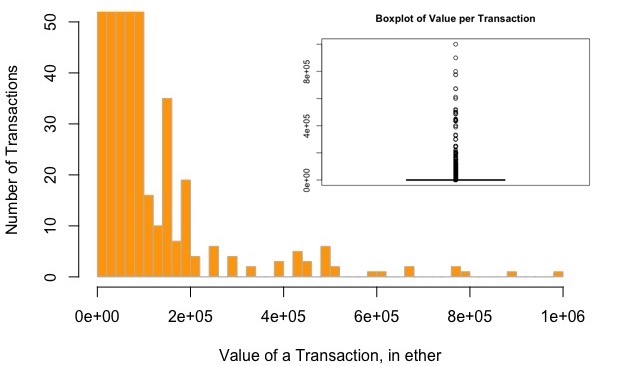
\includegraphics[width=\linewidth]{figures/value_per_tx.jpeg}
  \caption{Distribution of Value sent per Transaction.\\ 
  \textit{*The number of transactions on the Y axis is limited to 50, so that the less frequent values remain visible.}}
  \label{fig:value_per_tx}
\end{figure}

The spikes in the amount of fees paid in transactions (see Figure \ref{fig:fee_per_tx}) gives a hint at the underlying variation in businesses activity and Ethereum design issues.
Cryptocurrencies are often promoted as a fast medium for micro-payments. 
However, fast transactions with low fees are not always the case.
Limitations in the block size and the number of blocks in a period of time may result in an overflow of transactions pending to be included in a block.
To speed up transactions people pay higher fees.
At the same time, when the exchange rate of a cryptocurrecny rises, fees tend to become lower.

\begin{figure}[h]
  \centering
  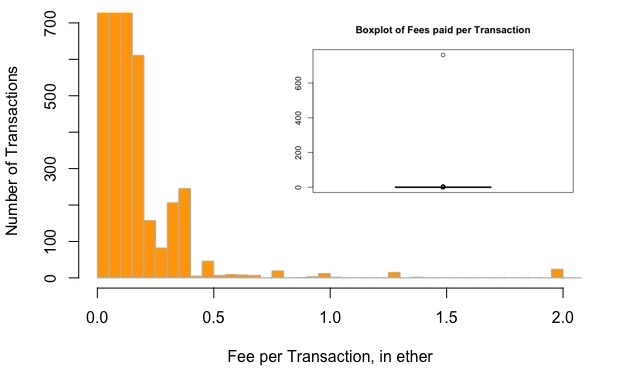
\includegraphics[width=\linewidth]{figures/fee_per_tx.jpeg}
  \caption{Distribution of Fees paid per Transaction.\\ 
  \textit{*The number of transactions on the Y axis is limited to 700, so that the less frequent fees remain visible.}}
  \label{fig:fee_per_tx}
\end{figure}

Interestingly, the is a big outlier - once there was a fee of more than 600 ether (80 000 U.S. dollars as of 15.03.2019).
Apparently this is due to a mistake made by a payer.
Such a mistake shows one of the disadvantages of the blockchain-based currencies where all transactions are irreversible.

Analysis of the distribution of gas used in transactions (see Figure \ref{fig:gas_per_tx}) points at differences in their types.
As gas measures how much "work" an action or a set of actions takes to perform, this potentially can be used to make a preliminary judgement about the prevalence of the smart contracts or about distribution of their complexity.

\begin{figure}[h]
  \centering
  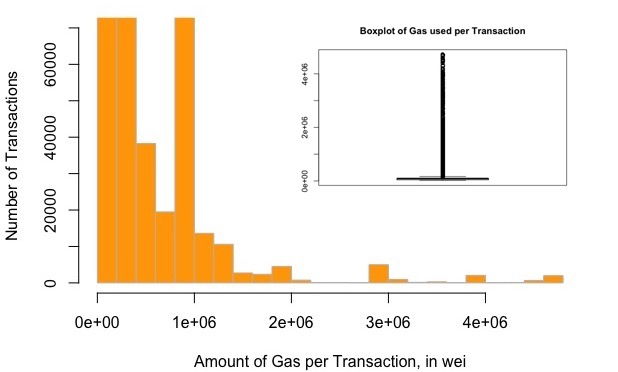
\includegraphics[width=\linewidth]{figures/gas_per_tx.jpeg}
  \caption{Distribution of Gas used per Transaction. \\ 
  \textit{*The number of transactions on the Y axis is limited to 70 000, so that the less frequent amount of gas remain visible.}}
  \label{fig:gas_per_tx}
\end{figure}

There are obviously two major clusters that probably separate regular payment transactions and smart contracts plus several groups of more complex contracts that however represent minority in the total volume of transactions. 
Both median and the 3rd quartile amount of gas is equal to 90 000 wei. In case the above hypothesis is correct, regular payment transactions will cover at least 75 \% of the total number and are all represented on the Figure \ref{fig:gas_per_tx} by the 1st bar (cut in order to make other values visible).

Analysis of the transactions number over time makes the concern about unequal distribution of wealth in the network visible. 
As illustrated on the Figure \ref{fig:tx_over_time} the number of transactions on the most active days more than doubles the respective number on the days with the lowest activity. 
Such significant variation indicates at the presence of major nodes.  

\begin{figure}[h]
  \centering
  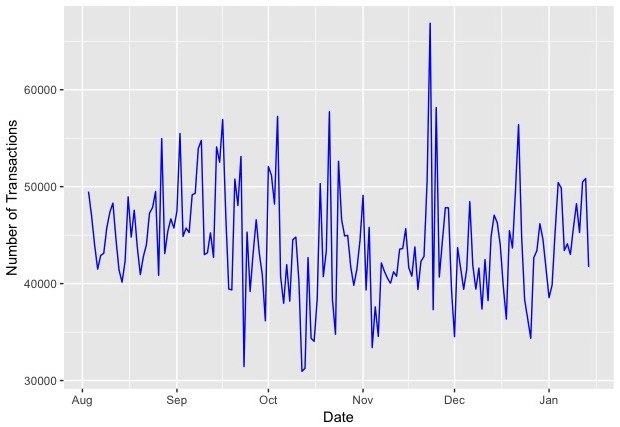
\includegraphics[width=\linewidth]{figures/tx_over_time.jpeg}
  \caption{Number of Transactions over Time.}
  \label{fig:tx_over_time}
\end{figure}

This becomes even more visible if we consider the monetary volume of transactions over time (see Figure \ref{fig:volume_over_time}).
Increases in volume of up to a hundred times from one day to another are an example of activity that would lead to a drastic changes in prices if these transactions are made not on chain but on currency exchanges.

\begin{figure}[h]
  \centering
  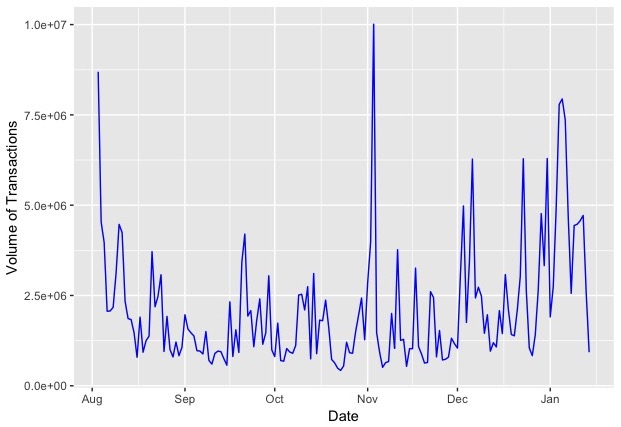
\includegraphics[width=\linewidth]{figures/volume_over_time.jpeg}
  \caption{Volume of Transactions over Time, in ether.}
  \label{fig:volume_over_time}
\end{figure}

\begin{figure*}[h]
  \centering
  \begin{subfigure}[b]{0.49\linewidth}
    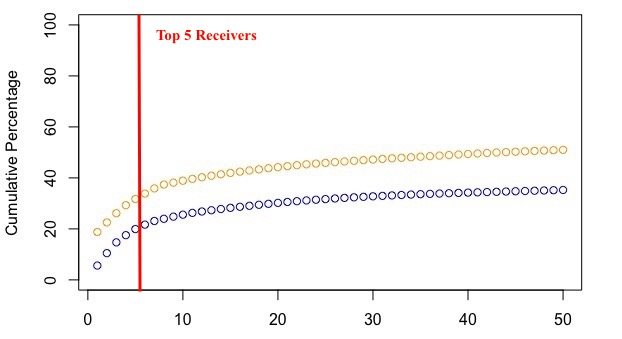
\includegraphics[width=\linewidth]{figures/major_receivers_metrics.jpeg}
    \caption{Top 50 Receivers.}
    \label{fig:major_receivers_metrics}
  \end{subfigure}
  \begin{subfigure}[b]{0.49\linewidth}
    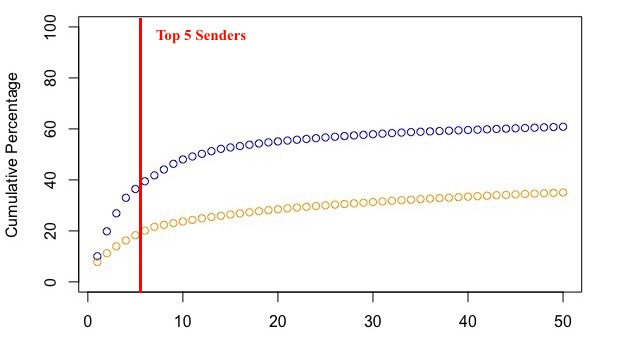
\includegraphics[width=\linewidth]{figures/major_senders_metrics.jpeg}
    \caption{Top 50 Senders.}
    \label{fig:major_senders_metrics}
  \end{subfigure}
  \caption{Cumulative Percentage of Transactions (blue) and Volume (orange) covered by Major Receivers (a) and Senders (b).}
  \label{fig:major_metrics}
\end{figure*}

In order to verify the hypothesis about the presence of major nodes we analyse transactions number and volume more in depth. 
This is done by associating transactions with individual accounts.
We treat receivers and senders of transactions separately.

As shown on the Figure \ref{fig:major_receivers_metrics} top 5 major accounts have received 19,9 \% of all transactions (1,45 out of 7,3 million transactions).
Top 50 accounts cover slightly more than one third of the total transactions' number.
When it comes to the monetary value, the situation is even more centralized.
Top 5 accounts have received 31,8 \% of the total transactions' value (112 out of 352 million ether received in all transactions).
Major 50 Receivers cover more than a half of the volume transacted within the network. 

Figure \ref{fig:major_senders_metrics} shows the data for major senders of transactions.
Here, in terms of the transactions' number the situation is even more centralized.
Top 5 accounts have made 36,4 \% of all transactions.
Top 50 senders cover 60,1 \% of the entire transactions' number.
At the same time in terms of volume the picture is different.
Top 5 and Top 50 senders cover only 18,3 \% and 35,0 \% of the total transactions' value respectively.

Interestingly, there are significant discrepancies in the degree of centralization if the data about receivers and spenders is compared to each other.
This is the case for centralization both in terms of transactions' number and volume.
Analysis of these discrepancies may shade light on some of the roles that major nodes play in the network.

\textit{Discrepancies in the Transactions' Volume between Receivers and Senders.} 
There is a significant difference between the amount of ether received and spent by the major accounts.
While Top 50 Receivers have accumulated 172 million ether, Top 50 Senders have spent only 123 million.
Besides, top receivers and senders should not necessarily be the same entities. 
Consequently there is a number of major nodes that spend less than their receive or don't spend at all.
Figure \ref{fig:balances} shows the net balances of the accounts within the studied period of time. 
While absolute majority of accounts have balance around 0, there are few that have accumulated a significant amount of wealth.

\begin{figure}[h!]
  \centering
  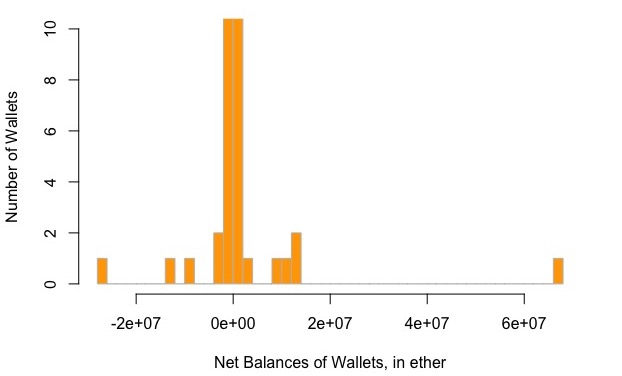
\includegraphics[width=1\linewidth]{figures/balances.jpeg}
  \caption{Distribution of Balances within Studied Period. \\ 
  \textit{*The number of wallets on the Y axis is limited to 10, so that the less frequent wallets remain visible.}}
  \label{fig:balances}
\end{figure}

Those could be mining pools that receive new coins and hold them anticipating appreciation of ether.
However the amount of Ethereum accumulated by such nodes seems to be too big to be explained this way.
Despite a new block in Ethereum is mined every 10-20 seconds and remunerates miners with 5 ether, during the analyzed period of time this results in only approximately 5 million new ether.

Probably, these nodes are currency exchanges that accumulate wealth of their participants. 
They keep track of exchange transactions internally without recording them on-chain. 
The wealth is recorded as spent only when a participant makes a payment transaction.

If the nodes are actually currency exchanges, there is a deviation from the Ethereum narrative of "no trusted third party involvement".
Given the level of centralization associated with the nodes, this could imply a major source of vulnerability.
An attack on the exchange records would lead to losses for a significant number of the exchange participants.

\begin{table*}
\centering
\captionof{table}{Top 5 Major Receivers (Volume)} 
\label{tab:t5mr} 
\begin{adjustbox}{width=0.9\linewidth}
% \small
% \resizebox{\columnwidth}{!}{%
\begin{tabular}{lccl}
% \begin{tabulary}{\linewidth}{RLRR}
  \hline
Wallet & Amount Received, mill. ether & Type & Affiliation \\
  \hline
  0xAA1A6e3e6EF20068f7F8d8C835d2D22fd5116444 & 66,0 & Smart-Contract & ReplaySafeSplit \\ 
  0xBFC39b6F805a9E40E77291afF27aeE3C96915BDD & 13,2 & Smart-Contract & Poloniex \\ 
  0x209c4784AB1E8183Cf58cA33cb740efbF3FC18EF & 12,6 & Smart-Contract & Poloniex 2 \\ 
  0x7727E5113D1d161373623e5f49FD568B4F543a9E & 11,1 & Smart-Contract & Bitfinex 2 \\ 
  0xFa52274DD61E1643d2205169732f29114BC240b3 & 8,5 & Smart-Contract & Kraken 4 \\ 
   \hline
% \end{tabulary}
\end{tabular}
\end{adjustbox}
% }
\end{table*}

\begin{table*}
\centering
\captionof{table}{Top 5 Major Senders (Number of TXs)}
\label{tabt5ms}
\begin{adjustbox}{width=0.9\linewidth}
\begin{tabular}{p{7cm}ccl}
  \hline
Wallet & Number of TXs send & Type & Affiliation \\
  \hline
  0xEA674fdDe714fd979de3EdF0F56AA9716B898ec8 & 733818 & Address & Ethermine \\
  0x2a65Aca4D5fC5B5C859090a6c34d164135398226 & 715017 & Address & DwarfPool 1 \\
  0xD34DA389374CAAD1A048FBDC4569AAE33fD5a375 & 516932 & Address & GenesisMining \\
  0x52bc44d5378309EE2abF1539BF71dE1b7d7bE3b5 & 443544 & Address & Nanopool \\
  0x61C808D82A3Ac53231750daDc13c777b59310bD9 & 251566 & Address & F2Pool 1 \\
   \hline
\end{tabular}
\end{adjustbox}
\end{table*}

In order to verify how relevant this risk actually is, we conducted further investigation of the accounts that received the biggest volumes of ether.  
Using data of the Ethereum scanners such as Etherscan.io, Etherchain.org, Blockchair.com, Bloxy.info, etc.\footnote{For details see: \\ \url{https://etherscan.io/}, \\ \url{https://www.etherchain.org/}, \\ \url{https://blockchair.com/Ethereum/}, \\ \url{https://bloxy.info/}.} we found out affiliation of the Top 5 Receivers (in terms of volume).

Four out of five Top Receivers actually belong to the currency exchanges (see Table \ref{tab:t5mr}).
However, all these accounts in reality appeared to be not regular addresses but smart contracts.
The remaining Top Receiver (the first one in the list) is also a smart contract.
None of them is supposed to accumulate wealth and by design should transfer it further.
This puts under question the validity or completeness of the transactions´ data we have collected.

Deeper research allowed restoring the faith in the dataset.
Appeared that money received by identified major accounts was actually spent.
Bit in another network.

The point is that on the 20th of July 2016 (shortly before the analyzed period) Ethereum experienced a hard fork.
As a consequence of the DAO incident - a hack of a complicated smart-contract that resulted in a loss of about 12.7 million ether (worth around 150 million U.S. dollars at the time) - the community was split in two parts.
Most of the network participants decided to make a fork chain where the stolen coins would be returned to their owners.
However, some of the community decided to continue the old chain (Ethereum Classic or ETC), arguing that "the code is the law" and the blockchain data should be irreversible\footnote{See for instance \url{https://www.cryptocompare.com/coins/guides/the-dao-the-hack-the-soft-fork-and-the-hard-fork/}.}.

This lead to a number of issues related to the interaction between chains.
One of the most relevant of them was "replay attack".
The mechanics of it is as follows:
if there is a valid transaction on one chain, it can also be offered - replayed - on the other chain to duplicate the received amount.
For instance, a user of the currency exchange can deposit and withdraw her money from this exchange on the old chain, and then use the 2nd transaction to withdraw money also on the new (forked) chain\footnote{See for instance \url{https://vessenes.com/hard-fork-and-replay-concerns/}.}.
This concern was solved through inter-mediation of the smart contracts.

Thus, the post by Ethereum founder Vitalik Buterin states:
"users who are interested in taking any actions with their ETC, including creating and participating in applications, converting to another asset, etc. are advised to use the splitter contract at address 0xAA1A6e3e6EF20068f7F8d8C835d2D22fd5116444 to move their ETC to a separate newly created account so as to avoid replay attacks; we also encourage the ETC community to consider adopting a secondary hard fork to change transaction formats to make further replay attacks impossible\footnote{For details see \url{https://blog.Ethereum.org/2016/07/26/onward\_from\_the\_hard\_fork/}.}.

The address mentioned in the post is the biggest Receiver in our dataset\footnote{The original address in the post was substituted as the original smart-contract was changed.}.
It has transmitted all the received money to its senders, but on the other chain.
The other 4 accounts, which are intermediate exchange wallets were apparently performing similar function of splitting wealth between different chains.

Thus, our concern about possible attack is confirmed only partially.
None of the Top 5 Receivers were accumulating wealth and it all was automatically transmitted to other accounts.
At the same time while exploring the "ReplaySafeSplit" smart-contract we have found that a number of users lost their money due to the mistakes made by them during the split\footnote{See for instance \url{https://medium.com/@chevdor/safer-version-of-the-replaysafesplit-smart-contract-a29c347e8a7}.}.
The smart-contract itself appeared to be susceptible to a number of bugs\footnote{For details see \url{https://etherscan.io/address/0xaa1a6e3e6ef20068f7f8d8c835d2d22fd5116444\#code}.} and was later substituted by another one.
The DAO incident described in the context of our Receivers exploration also exemplifies how the risk of the attack on an account or contract that holds funds from different users can and has actually played out.

\textit{Discrepancies in the Transactions' Number between Receivers and Senders.} 
As has been described by the Figure \ref{fig:major_metrics} the number of transactions received by major Receivers is significantly smaller than the number of transactions made by major Senders.
This discrepancy can probably be partially explained by the activity of the mining pools.
There, one account receives a mining reward and then sends it in small fractions to the many participants of the pool.

Alternative explanation can be related to various approaches of the network participants to gain more privacy.
One of them is the so called "peeling-chain".
The technique consists in dividing and sending the wealth of an account to multiple addresses again and again.
The goal is to create an impression that several users are doing transactions instead of one.

The process is illustrated on the Figure \ref{fig:peeling_chain}.
Here, the received amount of 50 coins is splitted in several iterations to multiple accounts in an attempt to complicate tracking of a certain person´s wealth.

\begin{figure}[h]
  \centering
  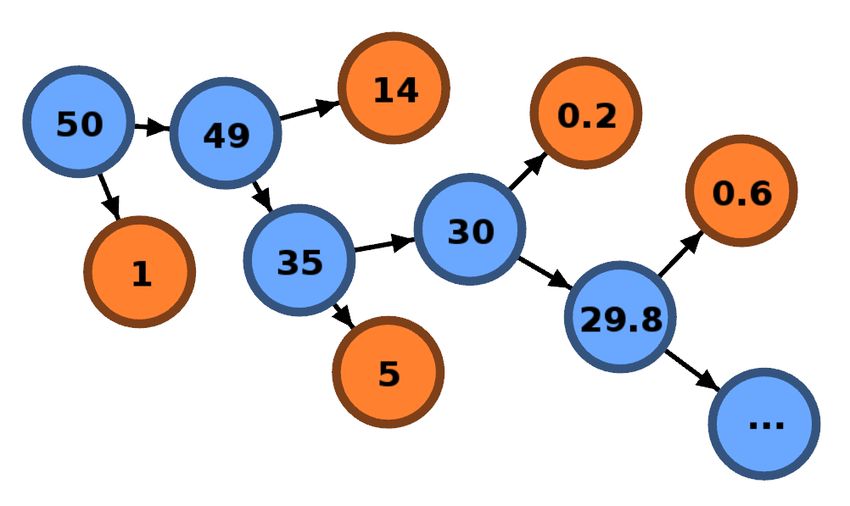
\includegraphics[width=\linewidth]{figures/peelingchain.png}
  \caption{How the peeling-chain works. From \cite{balthasar2017laundary}}
  \label{fig:peeling_chain}
\end{figure}

Further research of the Top 5 transaction Senders allowed verifying the hypotheses about the role of different nodes and their activities.
Using data of the Ethereum scanners as before we disclosed identities of the major accounts. 
All of them appeared to be mining pools (see Table \ref{tabt5ms}.
Among Top 5 Receivers of transactions there are no mining pools (the accounts are a digital token YoCoin, 2 Poloniex exchange wallets, currently closed by the U.S. government cryptocurrency trading platform BTC-e and already mentioned ReplaySafeSplit smart-contract).
Thus the hypothesis about the activity of mining pools is confirmed.
"Peeling-chain" practices are neither confirmed nor disproved.

% Accounts receiving major number of transactions were rarely (only ..times) seen in the list of major senders





% \begin{figure}
%   \centering
%   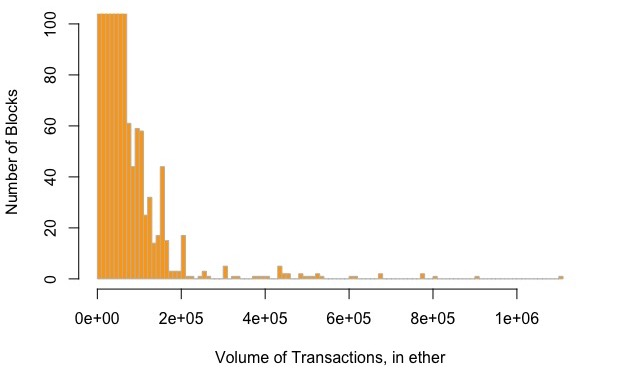
\includegraphics[width=\linewidth]{figures/volume_per_block.jpeg}
%   \caption{Distribution of Transactions' Volume per Block.}
%   \label{fig:volume_per_block}
% \end{figure}

